\documentclass[10pt]{beamer}
\usetheme{metropolis}

% ── Packages ──
\usepackage{amsmath,amssymb,amsthm}
\usepackage{tikz}
\usetikzlibrary{positioning,arrows.meta,fit,matrix,backgrounds,calc,shapes.geometric}
\usepackage{graphicx}
\usepackage{array}
\usepackage{etoolbox}

% ── Theorem environments ──
\theoremstyle{definition}
\newtheorem{defi}{Definition}[section]
\newtheorem{prop}{Proposition}[section]
\newtheorem{thm}{Theorem}[section]
\newtheorem{cor}{Corollary}[section]

% Custom theorem styles with colors
\setbeamercolor{block title}{bg=red!75!black,fg=white}
\setbeamercolor{block body}{bg=yellow!10!white}

% Proposition uses yellow title
\AtBeginEnvironment{prop}{%
  \setbeamercolor{block title}{bg=yellow!75!black,fg=black}%
  \setbeamercolor{block body}{bg=yellow!10!white}%
}
\AtEndEnvironment{prop}{%
  \setbeamercolor{block title}{bg=red!75!black,fg=white}%
}

% Theorem uses yellow title
\AtBeginEnvironment{thm}{%
  \setbeamercolor{block title}{bg=yellow!75!black,fg=black}%
  \setbeamercolor{block body}{bg=yellow!10!white}%
}
\AtEndEnvironment{thm}{%
  \setbeamercolor{block title}{bg=red!75!black,fg=white}%
}

% Corollary uses yellow title
\AtBeginEnvironment{cor}{%
  \setbeamercolor{block title}{bg=yellow!75!black,fg=black}%
  \setbeamercolor{block body}{bg=yellow!10!white}%
}
\AtEndEnvironment{cor}{%
  \setbeamercolor{block title}{bg=red!75!black,fg=white}%
}

% ── Highlighting ──
\newcommand{\x}[1]{\alert{\textbf{#1}}}

% ── Cross-filling colors ──
\newcommand{\pvt}[1]{{\color{red}\mathbf{#1}}}       % pivot
\newcommand{\crs}[1]{{\color{blue}#1}}                % cross arm
\newcommand{\ghost}[1]{{\color{yellow!50!black}#1}}   % cleared cross (muted complement of blue)
\newcommand{\bl}[1]{{\color{blue}#1}}                 % blue highlight (R₁)
\newcommand{\rd}[1]{{\color{red!70!black}#1}}         % red highlight (R₂)
\newcommand{\tl}[1]{{\color{teal}#1}}                 % teal highlight (R₃)

\title{Lecture 8: Cross-Filling Projections}
\subtitle{MATH203 Applied Linear Algebra}
\date{}

\begin{document}
\maketitle

% ═══════════════════════════════════════
% §1 CROSS-FILLING A PROJECTION — ACT 1: DISCOVERY
% ═══════════════════════════════════════
%
% ADR: The audience enters with two tools from previous lectures:
%   - Projections (P² = P) from Lecture 7
%   - Cross-filling (any matrix = sum of rank-1 pieces) from Lecture 3
% We DO NOT preview the theorem. Instead, we pose a concrete exercise
% ("compute the rank of this projection") that forces cross-filling.
% At each step, the audience discovers something surprising: the pieces
% and remainders are all projections too. The pattern builds over three
% steps until the audience is thinking "this can't be a coincidence."
% ONLY THEN do we ask "why?" — tension at its peak.
%
% WHY NOT PREVIEW: Telling the audience "each piece is a projection"
% before they compute kills the discovery. They verify instead of
% discover. Verification is passive; discovery is active.
\section{Cross-Filling a Projection}

% ADR: Open with a concrete exercise, not a theorem. The audience thinks
% they are doing routine rank computation. The surprise comes mid-computation.
% AUDIENCE EMOTION: "ok, I know how to do this" (confidence, low stakes)
% AUDIENCE ATTENTION: active — they are computing along with us.
\begin{frame}{Exercise: Compute the Rank}

The following matrix is a projection ($P^2 = P$).

\vspace{0.3em}

$$P = \begin{pmatrix} 0 & 0 & 0 & 0 \\ -2 & 1 & 0 & 0 \\ 1 & 0 & 1 & 0 \\ -1 & 0 & 0 & 1 \end{pmatrix}$$

\vspace{0.3em}

\x{Task}: Compute $\operatorname{rank}(P)$ by cross-filling.

\end{frame}

% ADR: Step 1 — routine cross-filling. Nothing surprising yet.
% The audience is in "computation mode." We show the mechanics.
\begin{frame}{Cross-Filling: Step 1}

$P_{(1,1)} = 0$ --- skip. \quad \x{First pivot} at $(2,2)$, value $= \pvt{1}$:

$$P = \begin{pmatrix} 0 & \crs{0} & 0 & 0 \\ \crs{-2} & \pvt{1} & \crs{0} & \crs{0} \\ 1 & \crs{0} & 1 & 0 \\ -1 & \crs{0} & 0 & 1 \end{pmatrix}$$

$$R_1 = \frac{1}{\pvt{1}}\begin{pmatrix} \crs{0} \\ \crs{1} \\ \crs{0} \\ \crs{0} \end{pmatrix} \begin{pmatrix} \crs{-2} & \crs{1} & \crs{0} & \crs{0} \end{pmatrix}
= \begin{pmatrix} 0 & \crs{0} & 0 & 0 \\ \crs{-2} & \pvt{1} & \crs{0} & \crs{0} \\ 0 & \crs{0} & 0 & 0 \\ 0 & \crs{0} & 0 & 0 \end{pmatrix}$$

\end{frame}

% ADR: Explicitly write out P = R₁ + (P - R₁) with concrete matrices and
% underbrace labels. This is NOT redundant — it serves two critical purposes:
%   (1) The audience needs to SEE the decomposition laid out to process it.
%       Jumping from "here is R₁" to "is R₁² = R₁?" skips a cognitive step:
%       the audience hasn't yet absorbed what the remainder looks like.
%   (2) The underbrace labels (R₁ and "remainder") give the two pieces
%       identities that the audience can track. When we later ask "is R₁ a
%       projection? is the remainder a projection?", they know exactly which
%       matrix we mean.
%   Without this slide, the audience is doing subtraction in their head while
%   simultaneously trying to follow the next argument. Cognitive overload.
%
%   CROSS HIGHLIGHTING inside R₁ and remainder:
%   R₁ shows the (2,2)-cross in blue/red — this is the visual origin story:
%   "this piece IS the cross extracted from P." The audience sees the same
%   color pattern they saw on the previous slide, now isolated into its own
%   matrix. Without this, R₁ is just a matrix of numbers with no visual link
%   to the cross-filling operation that produced it.
%   The remainder shows the SAME (2,2)-cross — but in a muted yellow
%   (\ghost), the visual complement/inverse of blue. Every entry on that
%   cross is ZERO. The color contrast tells the story instantly:
%     blue cross in R₁ = "the values live here"
%     yellow ghost in remainder = "the values were here, now gone"
%   This is the visual payoff: "the cross was surgically extracted, leaving
%   nothing behind." The cleanness is not cosmetic — it is directly connected
%   to the mutual annihilation property (R₁ · remainder = 0) that the
%   audience will discover later. The muted yellow avoids confusion with
%   the blue that always means "active cross arm", while still marking the
%   same positions so the audience can visually track the before/after.
%
% AUDIENCE EMOTION: "ok, I see the two pieces clearly now"
% AUDIENCE ATTENTION: visual — colored cross patterns are eye-catching and
%   give the audience something concrete to anchor on in each matrix.
\begin{frame}{Cross-Filling: Step 1 --- The Decomposition}

$$P = \underbrace{\begin{pmatrix} 0 & \crs{0} & 0 & 0 \\ \crs{-2} & \pvt{1} & \crs{0} & \crs{0} \\ 0 & \crs{0} & 0 & 0 \\ 0 & \crs{0} & 0 & 0 \end{pmatrix}}_{R_1} + \underbrace{\begin{pmatrix} 0 & \ghost{0} & 0 & 0 \\ \ghost{0} & \ghost{0} & \ghost{0} & \ghost{0} \\ 1 & \ghost{0} & 1 & 0 \\ -1 & \ghost{0} & 0 & 1 \end{pmatrix}}_{\text{remainder}}$$

\vspace{0.5em}

A rank-1 piece, plus what's left. Standard cross-filling.

\vspace{0.5em}

But let's look more carefully at these two pieces\ldots

\end{frame}

% ADR: The DISCOVERY moment. We pause mid-computation to notice something.
% "Wait — R₁² = R₁?" This should feel like an accident the audience catches.
% We also check the remainder and find it is ALSO a projection.
% The audience has just SEEN both matrices on the previous slide, so they
% can immediately engage with the verification — no mental subtraction needed.
% AUDIENCE EMOTION: surprise — "that's weird, is that a coincidence?"
% AUDIENCE ATTENTION: spiked — pattern recognition is engaging.
\begin{frame}{Wait --- $R_1$ Is a Projection?}

Let's check: is $R_1^2 = R_1$?

$$R_1^2 = \begin{pmatrix} 0 & \crs{0} & 0 & 0 \\ \crs{-2} & \pvt{1} & \crs{0} & \crs{0} \\ 0 & \crs{0} & 0 & 0 \\ 0 & \crs{0} & 0 & 0 \end{pmatrix}^2 = \begin{pmatrix} 0 & \crs{0} & 0 & 0 \\ \crs{-2} & \pvt{1} & \crs{0} & \crs{0} \\ 0 & \crs{0} & 0 & 0 \\ 0 & \crs{0} & 0 & 0 \end{pmatrix} = R_1 \quad \checkmark$$

\vspace{0.3em}

And the \x{remainder} $P - R_1$?

$$\begin{pmatrix} 0 & \ghost{0} & 0 & 0 \\ \ghost{0} & \ghost{0} & \ghost{0} & \ghost{0} \\ 1 & \ghost{0} & 1 & 0 \\ -1 & \ghost{0} & 0 & 1 \end{pmatrix}^2 = \begin{pmatrix} 0 & \ghost{0} & 0 & 0 \\ \ghost{0} & \ghost{0} & \ghost{0} & \ghost{0} \\ 1 & \ghost{0} & 1 & 0 \\ -1 & \ghost{0} & 0 & 1 \end{pmatrix} \quad \checkmark$$

\vspace{0.3em}

The rank-1 piece \x{and} the remainder are \x{both projections}. Coincidence?

\end{frame}

% ADR: Step 2 — the audience is now watching for the pattern.
% They expect R₂ to also be a projection. We confirm it.
% AUDIENCE EMOTION: "it's happening again — this is a real pattern"
\begin{frame}{Cross-Filling: Step 2}

\x{Second pivot} at $(3,3)$, value $= \pvt{1}$ (in the remainder):

$$P - R_1 = \begin{pmatrix} 0 & 0 & \crs{0} & 0 \\ 0 & 0 & \crs{0} & 0 \\ \crs{1} & \crs{0} & \pvt{1} & \crs{0} \\ -1 & 0 & \crs{0} & 1 \end{pmatrix}$$

$$R_2 = \frac{1}{\pvt{1}}\begin{pmatrix} \crs{0} \\ \crs{0} \\ \crs{1} \\ \crs{0} \end{pmatrix} \begin{pmatrix} \crs{1} & \crs{0} & \crs{1} & \crs{0} \end{pmatrix}
= \begin{pmatrix} 0 & 0 & \crs{0} & 0 \\ 0 & 0 & \crs{0} & 0 \\ \crs{1} & \crs{0} & \pvt{1} & \crs{0} \\ 0 & 0 & \crs{0} & 0 \end{pmatrix}$$

\end{frame}

% ADR: Same decomposition view as Step 1 — show R₂ with its (3,3)-cross
% in blue/red, and the new remainder with ALL previously extracted crosses
% ghosted in yellow. The remainder after step 2 has been "bullied" by BOTH
% R₁ and R₂, so the ghost region is the UNION of the (2,2)-cross and the
% (3,3)-cross. This accumulating ghost pattern visually shows how each step
% carves away more of the matrix — the yellow region grows with each step.
% AUDIENCE ATTENTION: the growing yellow region is visually striking and
% reinforces the iterative nature of cross-filling.
\begin{frame}{Cross-Filling: Step 2 --- The Decomposition}

$$P - R_1 = \underbrace{\begin{pmatrix} 0 & 0 & \crs{0} & 0 \\ 0 & 0 & \crs{0} & 0 \\ \crs{1} & \crs{0} & \pvt{1} & \crs{0} \\ 0 & 0 & \crs{0} & 0 \end{pmatrix}}_{R_2} + \underbrace{\begin{pmatrix} 0 & \ghost{0} & \ghost{0} & 0 \\ \ghost{0} & \ghost{0} & \ghost{0} & \ghost{0} \\ \ghost{0} & \ghost{0} & \ghost{0} & \ghost{0} \\ -1 & \ghost{0} & \ghost{0} & 1 \end{pmatrix}}_{\text{remainder}}$$

\vspace{0.5em}

$R_2^2 = R_2 \;\checkmark$ \quad Again a projection! And the remainder too.

\end{frame}

% ADR: Step 3 — by now the pattern is undeniable.
\begin{frame}{Cross-Filling: Step 3}

\x{Third pivot} at $(4,4)$, value $= \pvt{1}$ (in the remainder):

$$P - R_1 - R_2 = \begin{pmatrix} 0 & 0 & 0 & \crs{0} \\ 0 & 0 & 0 & \crs{0} \\ 0 & 0 & 0 & \crs{0} \\ \crs{-1} & \crs{0} & \crs{0} & \pvt{1} \end{pmatrix}$$

$$R_3 = \frac{1}{\pvt{1}}\begin{pmatrix} \crs{0} \\ \crs{0} \\ \crs{0} \\ \crs{1} \end{pmatrix} \begin{pmatrix} \crs{-1} & \crs{0} & \crs{0} & \crs{1} \end{pmatrix}
= \begin{pmatrix} 0 & 0 & 0 & \crs{0} \\ 0 & 0 & 0 & \crs{0} \\ 0 & 0 & 0 & \crs{0} \\ \crs{-1} & \crs{0} & \crs{0} & \pvt{1} \end{pmatrix}$$

\vspace{0.3em}

$R_3^2 = R_3 \;\checkmark$ \quad Every single piece is a projection.

\end{frame}

% ADR: Summary of discoveries. Now we lay out ALL the patterns the audience
% has seen, including ones they might not have noticed (annihilation, rank=trace).
% This is the moment the audience goes from "neat pattern" to "there must be
% a deep reason." Peak tension before Act 2.
% AUDIENCE EMOTION: awe — "this is too clean to be an accident"
\begin{frame}{What Just Happened?}

$$P = \underbrace{\begin{pmatrix} 0 & \bl{0} & 0 & 0 \\ \bl{-2} & \bl{1} & \bl{0} & \bl{0} \\ 0 & \bl{0} & 0 & 0 \\ 0 & \bl{0} & 0 & 0 \end{pmatrix}}_{R_1} + \underbrace{\begin{pmatrix} 0 & 0 & \rd{0} & 0 \\ 0 & 0 & \rd{0} & 0 \\ \rd{1} & \rd{0} & \rd{1} & \rd{0} \\ 0 & 0 & \rd{0} & 0 \end{pmatrix}}_{R_2} + \underbrace{\begin{pmatrix} 0 & 0 & 0 & \tl{0} \\ 0 & 0 & 0 & \tl{0} \\ 0 & 0 & 0 & \tl{0} \\ \tl{-1} & \tl{0} & \tl{0} & \tl{1} \end{pmatrix}}_{R_3}$$

\vspace{0.3em}

\x{Every piece is a projection}: $\bl{R_1^2 = R_1}$, \; $\rd{R_2^2 = R_2}$, \; $\tl{R_3^2 = R_3}$ \;\checkmark

\vspace{0.3em}

\x{Pieces annihilate each other}: $R_i R_j = 0$ for $i \neq j$ \;\checkmark

\vspace{0.3em}

\x{Rank equals trace}: $\operatorname{rank}(P) = 3 = 0 + 1 + 1 + 1 = \operatorname{trace}(P)$ \;\checkmark

\end{frame}

% ADR: Contrast with a non-projection. Same step-by-step format as the
% projection example — show the matrix with cross, do the cross-filling
% computation, show the result with cross. Then check R₁² = R₁ with full
% matrix multiplication. The audience needs to SEE the failure in the same
% visual language they just learned, so the contrast is immediate.
% AUDIENCE EMOTION: "so it really is about P² = P, not about cross-filling"
\begin{frame}{For Contrast: A Non-Projection}

Does this happen for \x{every} matrix? \quad \x{No!}

\vspace{0.3em}

$$A = \begin{pmatrix} \pvt{2} & \crs{4} \\ \crs{1} & 2 \end{pmatrix} \quad (\text{rank } 1, \text{ but } A^2 \neq A)$$

\x{Pivot} at $(1,1)$, value $= \pvt{2}$:

$$R_1 = \frac{1}{\pvt{2}}\begin{pmatrix} \crs{2} \\ \crs{1} \end{pmatrix} \begin{pmatrix} \crs{2} & \crs{4} \end{pmatrix}
= \begin{pmatrix} \pvt{2} & \crs{4} \\ \crs{1} & 2 \end{pmatrix}$$

Rank $= 1$, so $A = R_1$ (one piece, no remainder).

\end{frame}

% ADR: Contrast slide — cross-fill a NON-projection A = [[2,4],[1,2]] and
% show that NONE of the nice properties hold: R₁² ≠ R₁ (it's 4R₁),
% and rank ≠ trace (1 ≠ 4). This sharpens the audience's understanding:
% the magic is not in cross-filling itself, but in cross-filling a
% PROJECTION. Without this contrast, the audience might over-generalize.
% AUDIENCE EMOTION: "so it really IS about P²=P, not just cross-filling"
% AUDIENCE ATTENTION: the ✗ marks are visually striking after all the ✓'s.
\begin{frame}{For Contrast: Everything Fails}

\x{Is $R_1$ a projection?}

$$R_1^2 = \begin{pmatrix} 2 & 4 \\ 1 & 2 \end{pmatrix} \begin{pmatrix} 2 & 4 \\ 1 & 2 \end{pmatrix} = \begin{pmatrix} 8 & 16 \\ 4 & 8 \end{pmatrix} = \x{4}\,R_1 \neq R_1 \quad \times$$

\vspace{0.5em}

\x{Does rank $=$ trace?}

$$\underbrace{\operatorname{rank}(A) = 1}_{\text{one piece}} \qquad \underbrace{\operatorname{trace}(A) = 2 + 2 = 4}_{\text{sum of diagonal}} \qquad 1 \neq 4 \quad \times$$

\vspace{0.5em}

None of the nice properties hold --- because $A$ is \x{not a projection}.

\end{frame}

% ADR: Tension page. The audience has seen the pattern (3 steps of discovery)
% and the contrast (non-projection fails). Now we ask the question at peak
% tension. This is the bridge from Act 1 (discovery) to Act 2 (explanation).
% AUDIENCE EMOTION: "I need to know why"
% AUDIENCE ATTENTION: maximal — they are hooked.
\begin{frame}{}

\vspace{3em}

\begin{center}
{\Large \x{Why} does cross-filling a projection produce projections?}

\vspace{2em}

{\small What is the hidden structure that makes $P^2 = P$ so special?}
\end{center}

\end{frame}

% ═══════════════════════════════════════
% §2 THE PROOF: VU = I
% ═══════════════════════════════════════
%
% ADR: §2 answers the "why?" planted at the end of §1. The audience saw
% three cross-filling steps all produce projections and wants an explanation.
% The key insight: writing P = UV and using P² = P algebraically forces
% VU = I. This is proven in the abstract, then verified on the concrete
% example. We also show the UV factorization concretely FIRST (with colored
% columns in U and rows in V matching the cross-filling pieces from §1)
% before stating the abstract theorem. The colors — blue for piece 1, red
% for piece 2, teal for piece 3 — carry over from §1's cross highlighting
% to maintain visual continuity. The audience sees "same pieces, new format."
\section{Why It Works: $P = UV$ Implies $VU = I$}

% ADR: Bridge from Act 1 — before stating the abstract theorem, go back to
% the concrete example and write P = UV. The audience has seen the cross-
% filling pieces R₁, R₂, R₃. Now we collect the columns and rows into U
% and V. This gives the audience a CONCRETE instance of P = UV before we
% ask them to think abstractly about it.
% AUDIENCE EMOTION: "ok, I recognize these — they came from the cross-filling"
% AUDIENCE ATTENTION: re-engaged by returning to a familiar example.
%
% ADR: We MUST first restate P = R₁ + R₂ + R₃ with colored cross matrices
% (repeating from the summary slide) before writing P = UV. The audience
% cannot be expected to remember the pieces from 5 slides ago. Without
% restating, the jump to "collect into U and V" is a mystery — which columns?
% which rows? By showing the colored sum first, each Rᵢ = uᵢvᵢᵀ is visible,
% and the "collect columns into U, rows into V" step is a natural regrouping
% that the audience can follow with their eyes.
% This is the same principle as §1: never ask the audience to hold information
% from a previous slide in working memory. Restate what they need, THEN build.
\begin{frame}{Back to Our Example: $P = R_1 + R_2 + R_3$}

Recall the cross-filling decomposition:

$$P = \underbrace{\begin{pmatrix} 0 & \bl{0} & 0 & 0 \\ \bl{-2} & \bl{1} & \bl{0} & \bl{0} \\ 0 & \bl{0} & 0 & 0 \\ 0 & \bl{0} & 0 & 0 \end{pmatrix}}_{\bl{R_1}} + \underbrace{\begin{pmatrix} 0 & 0 & \rd{0} & 0 \\ 0 & 0 & \rd{0} & 0 \\ \rd{1} & \rd{0} & \rd{1} & \rd{0} \\ 0 & 0 & \rd{0} & 0 \end{pmatrix}}_{\rd{R_2}} + \underbrace{\begin{pmatrix} 0 & 0 & 0 & \tl{0} \\ 0 & 0 & 0 & \tl{0} \\ 0 & 0 & 0 & \tl{0} \\ \tl{-1} & \tl{0} & \tl{0} & \tl{1} \end{pmatrix}}_{\tl{R_3}}$$

\vspace{0.3em}

Each $R_i = \underbrace{\text{column} \div \text{pivot}}_{\mathbf{u}_i} \cdot \underbrace{\text{row}}_{\mathbf{v}_i^T}$. \quad Can we collect all columns and rows?

\end{frame}

% ADR: Now the P = UV slide. The audience has JUST seen the three colored
% pieces. We extract uᵢ (columns ÷ pivot) and vᵢᵀ (rows) and stack them
% into U and V. Color-code columns of U and rows of V to match the Rᵢ
% they came from, so the audience can visually trace the correspondence.
\begin{frame}{Collecting into $P = UV$}

Stack the columns into $U$, the rows into $V$:

$$P = \underbrace{\begin{pmatrix} \bl{0} & \rd{0} & \tl{0} \\ \bl{1} & \rd{0} & \tl{0} \\ \bl{0} & \rd{1} & \tl{0} \\ \bl{0} & \rd{0} & \tl{1} \end{pmatrix}}_{U\,:\, \text{columns} \div \text{pivot}} \underbrace{\begin{pmatrix} \bl{-2} & \bl{1} & \bl{0} & \bl{0} \\ \rd{1} & \rd{0} & \rd{1} & \rd{0} \\ \tl{-1} & \tl{0} & \tl{0} & \tl{1} \end{pmatrix}}_{V\,:\, \text{rows}}$$

\vspace{0.3em}

$\bl{\mathbf{u}_1}\bl{\mathbf{v}_1^T} = \bl{R_1}$, \quad $\rd{\mathbf{u}_2}\rd{\mathbf{v}_2^T} = \rd{R_2}$, \quad $\tl{\mathbf{u}_3}\tl{\mathbf{v}_3^T} = \tl{R_3}$

\end{frame}

% ADR: The key discovery — compute VU and find it equals I₃.
% This is the concrete "aha" moment that motivates the abstract theorem.
% We show the full matrix multiplication so the audience can verify.
% AUDIENCE EMOTION: surprise — "VU = I? That's suspiciously clean."
% AUDIENCE ATTENTION: the audience just saw VU computed to a clean identity,
% which is unexpected and demands explanation.
\begin{frame}{Compute $VU$}

$$VU = \begin{pmatrix} \bl{-2} & \bl{1} & \bl{0} & \bl{0} \\ \rd{1} & \rd{0} & \rd{1} & \rd{0} \\ \tl{-1} & \tl{0} & \tl{0} & \tl{1} \end{pmatrix} \begin{pmatrix} \bl{0} & \rd{0} & \tl{0} \\ \bl{1} & \rd{0} & \tl{0} \\ \bl{0} & \rd{1} & \tl{0} \\ \bl{0} & \rd{0} & \tl{1} \end{pmatrix} = \begin{pmatrix} \bl{1} & 0 & 0 \\ 0 & \rd{1} & 0 \\ 0 & 0 & \tl{1} \end{pmatrix} = I_3$$

\vspace{0.5em}

$VU = I_3$ \x{automatically}!

\vspace{0.5em}

Recall the non-projection: $VU = 4 \neq I_1$. \quad So this is about $P^2 = P$.

\vspace{0.5em}

Is $VU = I$ \x{always} true when $P$ is a projection?

\end{frame}

% ADR: NOW state the theorem. The audience has seen the concrete instance,
% felt the surprise, and is primed to ask "is this always true?"
% The theorem answers exactly that question — it lands at peak curiosity.
\begin{frame}{The Key Theorem}

\begin{thm}[$VU = I$ Automatic]
Let $P$ be a projection ($P^2 = P$). Suppose $P = UV$ where:
\begin{itemize}
\item $U$ is $n \times r$ with linearly independent columns
\item $V$ is $r \times n$ with linearly independent rows
\end{itemize}

Then $VU = I_r$ \x{automatically}.
\end{thm}

\vspace{1em}

This single identity explains \x{everything} we discovered in Act 1.

\end{frame}

% ADR: The proof is deliberately short — three lines. The audience just sat
% through 10+ slides of concrete computation; a long proof here would be
% deflating. The brevity IS the punchline: "all that richness, explained by
% three lines of algebra." Each step gets a bold label so the audience can
% follow the logic even if they zone out for a moment.
% AUDIENCE EMOTION: satisfaction — "that's elegant"
% AUDIENCE ATTENTION: focused — proof is short enough to hold in one glance.
% ALT REJECTED: multi-slide proof with intermediate steps. The audience has
% SEEN the concrete version; they don't need hand-holding on the algebra.
\begin{frame}{Proof: Three Lines}

Expand $P^2 = P$ using $P = UV$:

$$\underbrace{UV \cdot UV}_{P^2} = \underbrace{UV}_{P}$$

\vspace{0.3em}

\x{Step 1}: Left-cancel $U$ (columns of $U$ are linearly independent):

$$UVUV = UV \quad\Longrightarrow\quad VUV = V$$

\vspace{0.3em}

\x{Step 2}: Right-cancel $V$ (rows of $V$ are linearly independent):

$$VUV = V \quad\Longrightarrow\quad VU = I_r$$

\vspace{0.3em}

Done! The proof uses \x{only} $P^2 = P$ and cancellation. \qed

\end{frame}

% ADR: Transition from abstract theorem back to concrete. Rewrite U and V
% with column/row labels using three colors. This sets up the audience to
% SEE why VU = I implies Rᵢ² = Rᵢ and RᵢRⱼ = 0 — they need the
% dot-product interpretation of VU entries.
% AUDIENCE EMOTION: "now let's see what VU = I actually means for the pieces"
% AUDIENCE ATTENTION: re-engaged — back to concrete matrices after a proof.
\begin{frame}{Now We Can Explain Everything}

Write $P = UV$ with $VU = I_r$:

$$U = \begin{pmatrix} | & | & & | \\ \bl{\mathbf{u}_1} & \rd{\mathbf{u}_2} & \cdots & \tl{\mathbf{u}_r} \\ | & | & & | \end{pmatrix}, \qquad V = \begin{pmatrix} - & \bl{\mathbf{v}_1^T} & - \\ - & \rd{\mathbf{v}_2^T} & - \\ & \vdots & \\ - & \tl{\mathbf{v}_r^T} & - \end{pmatrix}$$

Each rank-1 piece: $\bl{R_1} = \bl{\mathbf{u}_1} \bl{\mathbf{v}_1^T}$, \; $\rd{R_2} = \rd{\mathbf{u}_2} \rd{\mathbf{v}_2^T}$, \; \ldots \; $\tl{R_r} = \tl{\mathbf{u}_r} \tl{\mathbf{v}_r^T}$

\end{frame}

% ADR: Expand VU entry-by-entry so the audience can READ the dot products
% from the matrix. The diagonal entries (same-color: vᵢᵀuᵢ = 1) and
% off-diagonal entries (cross-color: vᵢᵀuⱼ = 0) are the ONLY two facts
% needed for the next two slides (Rᵢ² = Rᵢ and RᵢRⱼ = 0). By isolating
% them visually in the VU matrix, the audience absorbs both facts at once
% and the subsequent proofs become one-liners.
% AUDIENCE EMOTION: "oh, I see — the diagonal is 1 and off-diagonal is 0"
% AUDIENCE ATTENTION: the colored matrix is visually striking; pattern jumps out.
% WHY three colors: the color match between VU entries and Rᵢ labels
% makes the connection immediate — no need to say "where i = j" verbally.
\begin{frame}{What Does $VU = I_r$ Look Like?}

$$VU = \begin{pmatrix}
\bl{\mathbf{v}_1^T}\bl{\mathbf{u}_1} & \bl{\mathbf{v}_1^T}\rd{\mathbf{u}_2} & \cdots & \bl{\mathbf{v}_1^T}\tl{\mathbf{u}_r} \\
\rd{\mathbf{v}_2^T}\bl{\mathbf{u}_1} & \rd{\mathbf{v}_2^T}\rd{\mathbf{u}_2} & \cdots & \rd{\mathbf{v}_2^T}\tl{\mathbf{u}_r} \\
\vdots & \vdots & \ddots & \vdots \\
\tl{\mathbf{v}_r^T}\bl{\mathbf{u}_1} & \tl{\mathbf{v}_r^T}\rd{\mathbf{u}_2} & \cdots & \tl{\mathbf{v}_r^T}\tl{\mathbf{u}_r}
\end{pmatrix} = \begin{pmatrix}
\bl{1} & 0 & \cdots & 0 \\
0 & \rd{1} & \cdots & 0 \\
\vdots & \vdots & \ddots & \vdots \\
0 & 0 & \cdots & \tl{1}
\end{pmatrix} = I_r$$

\vspace{0.3em}

\x{Diagonal}: $\mathbf{v}_i^T \mathbf{u}_i = 1$ \quad (same-color pairs multiply to 1)

\x{Off-diagonal}: $\mathbf{v}_i^T \mathbf{u}_j = 0$ for $i \neq j$ \quad (different-color pairs multiply to 0)

\end{frame}

% ADR: One-line proof using vᵢᵀuᵢ = 1 (diagonal of VU = I). The audience
% just saw this fact highlighted on the previous slide; now they see it
% "fire" in a computation. The underbrace "= 1" is the payoff moment.
% AUDIENCE EMOTION: "that's exactly what we just set up — it works!"
% AUDIENCE ATTENTION: the proof is short enough to verify mentally on the spot.
\begin{frame}{Each Piece Is a Projection}

\x{Goal}: Show $R_i^2 = R_i$ using $\bl{\mathbf{v}_i^T} \bl{\mathbf{u}_i} = 1$.

\vspace{0.5em}

$$R_i^2 = (\bl{\mathbf{u}_i} \bl{\mathbf{v}_i^T})(\bl{\mathbf{u}_i} \bl{\mathbf{v}_i^T}) = \bl{\mathbf{u}_i} \underbrace{(\bl{\mathbf{v}_i^T} \bl{\mathbf{u}_i})}_{= 1} \bl{\mathbf{v}_i^T} = \bl{\mathbf{u}_i} \bl{\mathbf{v}_i^T} = R_i \quad\checkmark$$

\vspace{0.5em}

Each cross-filling piece $R_i = \mathbf{u}_i \mathbf{v}_i^T$ is \x{automatically a rank-1 projection}!

\end{frame}

% ADR: Same one-line structure as "Each Piece Is a Projection" — uses the
% OFF-diagonal of VU = I (cross-color: vᵢᵀuⱼ = 0). The parallel structure
% reinforces that BOTH properties (Rᵢ² = Rᵢ and RᵢRⱼ = 0) come from the
% same place: VU = I. The summary at the bottom ties the bow on Act 2.
% AUDIENCE EMOTION: "everything clicks — both properties from one identity"
% AUDIENCE ATTENTION: closure — the summary signals the end of the explanation arc.
\begin{frame}{Mutually Annihilating Pieces}

\x{Goal}: Show $R_i R_j = 0$ (for $i \neq j$) using $\bl{\mathbf{v}_i^T} \rd{\mathbf{u}_j} = 0$.

\vspace{0.5em}

$$R_i R_j = (\bl{\mathbf{u}_i} \bl{\mathbf{v}_i^T})(\rd{\mathbf{u}_j} \rd{\mathbf{v}_j^T}) = \bl{\mathbf{u}_i} \underbrace{(\bl{\mathbf{v}_i^T} \rd{\mathbf{u}_j})}_{= 0} \rd{\mathbf{v}_j^T} = 0 \quad\checkmark$$

\vspace{1em}

\x{Summary}: For a projection $P = R_1 + \cdots + R_r$ (cross-filling decomposition):
\begin{itemize}
\item Each $R_i$ is a rank-1 projection ($R_i^2 = R_i$)
\item Different pieces annihilate ($R_i R_j = 0$ for $i \neq j$)
\end{itemize}

Both follow from the single identity $VU = I_r$.

\end{frame}

% ═══════════════════════════════════════
% §3 RANK = TRACE
% ═══════════════════════════════════════
%
% ADR: This section is a quick harvest — the audience already discovered
% rank = trace empirically in Act 1 (the "What Just Happened?" slide).
% Now we prove it in one line using VU = I and cyclic trace. The section
% is deliberately short (4 slides) because the audience has momentum from
% Act 2 and we don't want to slow down before the symmetric case in §4.
% WHY HERE (not in §2): rank = trace is a CONSEQUENCE, not part of the
% VU = I proof. Mixing it into §2 would blur the boundary between the
% core theorem and its applications.
\section{Rank Equals Trace for Projections}

% ADR: DEDICATED callback slide — do NOT cram the callback into the theorem
% slide. The audience has just finished §2 (abstract VU = I proof, five
% explanation slides). Their working memory is full of abstract symbols.
% We need to RESET their attention back to the concrete example before
% moving on. Show the full 4×4 matrix P with diagonal entries highlighted
% in blue, then visually sum them: 0+1+1+1 = 3 = rank. The audience
% re-engages by SEEING the numbers, not by being told "remember Act 1."
% A one-sentence callback is too weak — the audience needs the matrix in
% front of them to reactivate the pattern. This is the same "never ask
% the audience to hold information from a previous slide" principle from §1.
% AUDIENCE EMOTION: "oh right — we saw this! the diagonal adds up to the rank"
% AUDIENCE ATTENTION: re-engaged — concrete matrix after abstract slides.
% WHY A FULL SLIDE: the audience needs a cognitive reset between §2's
% abstract proofs and §3's new theorem. One sentence doesn't do it.
\begin{frame}{Remember This?}

Our projection from Act 1:

$$P = \begin{pmatrix} \bl{0} & 0 & 0 & 0 \\ -2 & \bl{1} & 0 & 0 \\ 1 & 0 & \bl{1} & 0 \\ -1 & 0 & 0 & \bl{1} \end{pmatrix}$$

\vspace{0.3em}

$$\operatorname{trace}(P) = \bl{0} + \bl{1} + \bl{1} + \bl{1} = 3 = \operatorname{rank}(P)$$

\vspace{0.5em}

The diagonal entries sum to the rank. \quad \x{Coincidence?}

\end{frame}

% ADR: Now the theorem + proof. The audience has JUST re-seen the concrete
% pattern on the previous slide. The theorem answers the question they are
% already asking ("is this always true?"). The proof is one line using
% trace(UV) = trace(VU) = trace(Iᵣ) = r — all from VU = I.
% AUDIENCE EMOTION: "so it IS always true — and VU = I explains it again!"
% AUDIENCE ATTENTION: the proof is short enough to absorb in one glance.
\begin{frame}{Rank Equals Trace}

\begin{thm}[Rank = Trace for Projections]
For any projection $P$ ($P^2 = P$):
$$\operatorname{rank}(P) = \operatorname{trace}(P)$$
\end{thm}

\textbf{Proof}:
Write $P = UV$ with $\operatorname{rank}(P) = r$. By the previous theorem, $VU = I_r$.

$$\operatorname{trace}(P) = \operatorname{trace}(UV) = \operatorname{trace}(VU) = \operatorname{trace}(I_r) = r = \operatorname{rank}(P)$$

Done --- one line from $VU = I$. \qed

\end{frame}

% ADR: Reframe the two utility facts as "the two extremes" of rank = trace.
% Instead of presenting them as isolated tool-lemmas ("we'll use these later"),
% position them as the natural boundary cases of the theorem we just proved:
%   - rank = trace = 0  →  the smallest projection is the zero matrix
%   - rank = trace = n  →  the largest projection is I
% This makes the slide a CONTINUATION of the rank = trace story rather than
% an interruption. The audience thinks "what are the edge cases?" — a natural
% follow-up to any theorem. The facts are still available for §5 proofs,
% but their motivation is now intrinsic, not forward-referencing.
% AUDIENCE EMOTION: "makes sense — rank = trace pins down the extremes"
% AUDIENCE ATTENTION: the two cases are symmetric and memorable.
% ALT REJECTED: old framing as "Two Quick Facts... we will use below."
% That framing made the audience feel these were unmotivated tool-deposits.
\begin{frame}{The Two Extremes}

What are the \x{smallest} and \x{largest} projections?

\vspace{0.5em}

\begin{prop}[The Smallest: $P = 0$]
If $P$ is a projection with $\operatorname{rank}(P) = 0$, then $P = 0$.
\end{prop}

$\operatorname{rank} = 0$ means every column is zero. $\quad\checkmark$

\vspace{0.5em}

\begin{prop}[The Largest: $P = I$]
If $P$ is an $n \times n$ projection with $\operatorname{trace}(P) = n$, then $P = I_n$.
\end{prop}

\textbf{Proof}: $I_n - P$ is a projection with $\operatorname{trace}(I_n - P) = n - n = 0$.

By rank $=$ trace: $\operatorname{rank}(I_n - P) = 0$, so $I_n - P = 0$. \qed

\end{frame}

% ADR: Contrast slide — lead with Act 1's familiar non-projection
% A = [[2,4],[1,2]] (rank 1, trace 4) so the audience reconnects to a
% matrix they already know fails. Then show additional examples. The Act 1
% callback is stronger than a fresh example because the audience already
% has emotional context ("that's the matrix where everything broke").
% AUDIENCE EMOTION: "right — rank ≠ trace was exactly what went wrong there"
% AUDIENCE ATTENTION: the table is scannable; familiar example anchors it.
\begin{frame}{Why Only for Projections?}

Remember our non-projection from Act 1?

\vspace{0.3em}

\begin{center}
\begin{tabular}{l|c|c|c}
& $\operatorname{rank}$ & $\operatorname{trace}$ & Equal? \\
\hline
$\begin{pmatrix} 2 & 4 \\ 1 & 2 \end{pmatrix}$ (\x{Act 1}, not projection) & 1 & 4 & \texttimes \\[0.5em]
$\begin{pmatrix} 3 & 0 \\ 0 & 0 \end{pmatrix}$ (not projection) & 1 & 3 & \texttimes \\[0.5em]
$\frac{1}{5}\begin{pmatrix} 1 & 2 \\ 2 & 4 \end{pmatrix}$ (projection) & 1 & 1 & \checkmark \\[0.5em]
Our $4 \times 4$ example (\x{Act 1}, projection) & 3 & 3 & \checkmark \\
\end{tabular}
\end{center}

\vspace{0.3em}

$\operatorname{rank} = \operatorname{trace}$ is a \x{fingerprint} of projection matrices.

\end{frame}

% ADR: Practical payoff — the audience can now read rank from the diagonal
% of any projection WITHOUT cross-filling. This is the "so what?" moment
% for rank = trace: it saves computation. The 5×5 example is large enough
% to make the point (cross-filling this would be tedious) but small enough
% to fit on one slide. Blue diagonal entries draw the eye to the trace sum.
% AUDIENCE EMOTION: "neat, a shortcut — I'll use this on homework"
% AUDIENCE ATTENTION: the exercise format re-engages active computation.
\begin{frame}{Quick Application: Read the Rank from the Diagonal}

\begin{exampleblock}{Exercise}
The following matrix is a projection ($P^2 = P$). What is its rank?

$$P = \begin{pmatrix} \bl{0} & 0 & 0 & 0 & 0 \\ -1 & \bl{1} & 0 & 0 & 0 \\ -1 & 0 & \bl{1} & 0 & 0 \\ -1 & 0 & 0 & \bl{1} & 0 \\ -1 & 0 & 0 & 0 & \bl{1} \end{pmatrix}$$
\end{exampleblock}

\vspace{0.5em}

\x{Answer}: $\operatorname{rank}(P) = \operatorname{trace}(P) = 0 + 1 + 1 + 1 + 1 = 4$.

\vspace{0.5em}

No cross-filling needed --- just read the diagonal!

\end{frame}

% ═══════════════════════════════════════
% §4 ORTHOGONAL PROJECTIONS
% ═══════════════════════════════════════
%
% ADR: Discovery-first structure, mirroring §1. The audience cross-fills a
% symmetric projection along the diagonal and discovers THREE things:
%   (1) row = column^T at every step (symmetry)
%   (2) each piece Rᵢ = wᵢwᵢ^T for some vector wᵢ (symmetric rank-1)
%   (3) the wᵢ's are orthonormal — an orthonormal basis of Col(P) for free
% We do NOT preview any of these observations. The audience discovers them
% mid-computation, just like in §1. The theorem comes AFTER the discovery.
%
% WHY SEPARATE SECTION: orthogonal projections have strictly more structure
% than general projections. The diagonal cross-filling → orthonormal basis
% result bridges from algebraic projections (§1-§3) to geometric
% orthogonal projections, setting up Lecture 9.
\section{Orthogonal Projections: Orthonormal Bases for Free}

% ADR: Bridge from §3. The narrative is NOT "what extra happens" (too passive).
% Instead, pose a TENSION: orthogonal projections carry extra structure
% (P^T = P), but our cross-filling pieces from §1 only inherited P² = P.
% Can we make the pieces ALSO inherit symmetry? The audience feels a gap
% between what P has and what the Rᵢ's have. Then the reveal: choosing
% diagonal pivots does exactly this. This is the tension → reveal engine.
% AUDIENCE EMOTION: "can we preserve symmetry? I want to know how"
% AUDIENCE ATTENTION: the gap between P's structure and Rᵢ's structure
% creates a concrete question the audience wants answered.
\begin{frame}{What About Orthogonal Projections?}

So far: cross-filling \x{any} projection gives rank-1 projections.

\vspace{0.5em}

But an \x{orthogonal projection} carries \x{more structure}: $P^2 = P$ \x{and} $P^T = P$.

\vspace{0.5em}

Our rank-1 pieces $R_i$ inherited $R_i^2 = R_i$. \quad Can they also inherit $R_i^T = R_i$?

\vspace{1em}

\x{Yes} --- if we choose pivots \x{on the diagonal}.

\vspace{0.5em}

Let's see why.

\end{frame}

% ADR: Exercise slide — show the 3×3 symmetric projection with both P² = P
% and P^T = P verified. The audience enters computation mode.
% Smaller matrix (3×3 vs 4×4 in §1) because the focus is on the NEW
% observations (symmetry), not on cross-filling mechanics.
% AUDIENCE EMOTION: "I know how to do this — let's go"
% AUDIENCE ATTENTION: active — exercise format engages.
\begin{frame}{Exercise: Cross-Fill Along the Diagonal}

$$P = \begin{pmatrix} 1 & 0 & 0 \\ 0 & \frac{1}{2} & \frac{1}{2} \\ 0 & \frac{1}{2} & \frac{1}{2} \end{pmatrix} \qquad P^2 = P \;\checkmark \qquad P^T = P \;\checkmark$$

\vspace{1em}

\x{Task}: Cross-fill $P$ using \x{diagonal pivots} only.

\vspace{0.5em}

(Rank $= \operatorname{trace} = 1 + \frac{1}{2} + \frac{1}{2} = 2$, so we expect 2 steps.)

\end{frame}

% ADR: Step 1 — routine diagonal cross-filling. Show P with the (1,1)-cross
% highlighted. Compute R₁. The KEY moment: the underbrace labels for column
% and row, with "row = column^T!" on the row. This is the first symmetry
% observation. The audience notices it but we don't make a big deal yet —
% just plant the seed. Show R₁ result with cross highlighting.
% AUDIENCE EMOTION: "huh, the row IS the column transposed — that's neat"
% AUDIENCE ATTENTION: computation mode; the "column^T!" label catches the eye.
\begin{frame}{Diagonal Cross-Filling: Step 1}

\x{Pivot} at $(\pvt{1},\pvt{1})$, value $= \pvt{1}$:

$$P = \begin{pmatrix} \pvt{1} & \crs{0} & \crs{0} \\ \crs{0} & \frac{1}{2} & \frac{1}{2} \\ \crs{0} & \frac{1}{2} & \frac{1}{2} \end{pmatrix}$$

$$R_1 = \frac{1}{\pvt{1}} \underbrace{\begin{pmatrix} \crs{1} \\ \crs{0} \\ \crs{0} \end{pmatrix}}_{\text{column}} \cdot \underbrace{\begin{pmatrix} \crs{1} & \crs{0} & \crs{0} \end{pmatrix}}_{\text{row} \;=\; \text{column}^T!} = \begin{pmatrix} \pvt{1} & \crs{0} & \crs{0} \\ \crs{0} & 0 & 0 \\ \crs{0} & 0 & 0 \end{pmatrix}$$

\end{frame}

% ADR: Decomposition slide — show P = R₁ + remainder with cross/ghost.
% Same visual language as §1: blue/red cross in R₁, ghost yellow for the
% cleared (1,1)-cross in the remainder. The audience can compare with §1's
% decomposition slides. Key observation: R₁ is SYMMETRIC — we state this
% and mark it with ✓. Second seed planted.
% AUDIENCE EMOTION: "same pattern as §1 — and the piece is symmetric too"
% AUDIENCE ATTENTION: the ghost yellow is familiar from §1.
\begin{frame}{Step 1 --- The Decomposition}

$$P = \underbrace{\begin{pmatrix} \pvt{1} & \crs{0} & \crs{0} \\ \crs{0} & 0 & 0 \\ \crs{0} & 0 & 0 \end{pmatrix}}_{R_1 \;\text{(symmetric } \checkmark\text{)}} + \underbrace{\begin{pmatrix} \ghost{0} & \ghost{0} & \ghost{0} \\ \ghost{0} & \frac{1}{2} & \frac{1}{2} \\ \ghost{0} & \frac{1}{2} & \frac{1}{2} \end{pmatrix}}_{\text{remainder (also symmetric } \checkmark\text{)}}$$

\vspace{0.5em}

$R_1$ is a projection ($R_1^2 = R_1$ \checkmark) --- as expected from \S1.

\vspace{0.3em}

But now $R_1$ is also \x{symmetric}: $R_1^T = R_1$ \checkmark.

\end{frame}

% ADR: Step 2 — cross-fill the remainder at (2,2). Ghost the union of
% previously extracted crosses (just (1,1)-cross here). Again highlight
% "row = column^T!" — now the audience has seen it TWICE, so the pattern
% is undeniable. Show R₂ result and note it is also symmetric.
% AUDIENCE EMOTION: "it happened again — row = column^T, piece is symmetric"
% AUDIENCE ATTENTION: the repeated "column^T!" label confirms the pattern.
\begin{frame}{Diagonal Cross-Filling: Step 2}

\x{Pivot} at $(\pvt{2},\pvt{2})$ in the remainder, value $= \pvt{\frac{1}{2}}$:

$$P - R_1 = \begin{pmatrix} \ghost{0} & \ghost{0} & \ghost{0} \\ \ghost{0} & \pvt{\frac{1}{2}} & \crs{\frac{1}{2}} \\ \ghost{0} & \crs{\frac{1}{2}} & \frac{1}{2} \end{pmatrix}$$

$$R_2 = \frac{1}{\pvt{\frac{1}{2}}} \underbrace{\begin{pmatrix} \crs{0} \\ \crs{\frac{1}{2}} \\ \crs{\frac{1}{2}} \end{pmatrix}}_{\text{column}} \cdot \underbrace{\begin{pmatrix} \crs{0} & \crs{\frac{1}{2}} & \crs{\frac{1}{2}} \end{pmatrix}}_{\text{row} \;=\; \text{column}^T!} = \begin{pmatrix} 0 & \crs{0} & 0 \\ \crs{0} & \pvt{\frac{1}{2}} & \crs{\frac{1}{2}} \\ 0 & \crs{\frac{1}{2}} & \frac{1}{2} \end{pmatrix}$$

Again: row $=$ column$^T$, and $R_2$ is \x{symmetric} $\checkmark$

\end{frame}

% ADR: Full-page discovery slide. The audience has seen row = column^T at
% every step. Now we draw the consequence: since Rᵢ = (column/pivot)·row
% and row = column^T, we can write Rᵢ = wᵢwᵢ^T where wᵢ = column/√pivot.
% Show the extraction for BOTH pieces explicitly — write out the formula,
% then the concrete vectors w₁ and w₂. The audience needs to SEE the
% vectors materialized, not just hear "normalize."
% AUDIENCE EMOTION: "so symmetric cross-filling gives us vectors for free!"
% AUDIENCE ATTENTION: high — the new wᵢ notation is the conceptual payoff.
\begin{frame}{Row $=$ Column$^T$ --- So What?}

Since row $=$ column$^T$, each piece factors as:

$$R_i = \frac{1}{\text{pivot}} \cdot \text{col} \cdot \text{col}^T = \underbrace{\frac{\text{col}}{\sqrt{\text{pivot}}}}_{\mathbf{w}_i} \cdot \underbrace{\frac{\text{col}^T}{\sqrt{\text{pivot}}}}_{\mathbf{w}_i^T} = \mathbf{w}_i \mathbf{w}_i^T$$

\vspace{0.2em}

\x{Step 1}: $\text{col} = \left(\begin{smallmatrix} 1 \\ 0 \\ 0 \end{smallmatrix}\right)$, $\text{pivot} = 1$ \quad $\Longrightarrow$ \quad $\mathbf{w}_1 = \begin{pmatrix} 1 \\ 0 \\ 0 \end{pmatrix}$

\vspace{0.2em}

\x{Step 2}: $\text{col} = \left(\begin{smallmatrix} 0 \\ 1/2 \\ 1/2 \end{smallmatrix}\right)$, $\text{pivot} = \frac{1}{2}$ \quad $\Longrightarrow$ \quad $\mathbf{w}_2 = \frac{1}{\sqrt{1/2}}\left(\begin{smallmatrix} 0 \\ 1/2 \\ 1/2 \end{smallmatrix}\right) = \begin{pmatrix} 0 \\ \frac{1}{\sqrt{2}} \\ \frac{1}{\sqrt{2}} \end{pmatrix}$

\end{frame}

% ADR: VISUAL IMPACT slide. Draw w₁ and w₂ as 3D vectors. The audience
% SEES them before any algebra: w₁ points along the x₁-axis, w₂ points
% into the x₂x₃-plane at 45°. They are VISUALLY perpendicular and both
% look like unit vectors. The audience's geometric intuition fires
% BEFORE we give any definitions. This is the discovery moment.
% AUDIENCE EMOTION: "wait... they're perpendicular? and unit length?"
% AUDIENCE ATTENTION: maximal — the picture is immediate and visceral.
% WHY PICTURE FIRST (Option B): see the geometry, THEN name it.
% If we define orthonormal first, the picture becomes verification.
% If we show the picture first, the definition gives vocabulary for
% something the audience already intuits. Discovery > verification.
\begin{frame}{Let's Draw Them}

$P = \mathbf{w}_1\mathbf{w}_1^T + \mathbf{w}_2\mathbf{w}_2^T$, \quad where $\mathbf{w}_1 = \left(\begin{smallmatrix} 1 \\ 0 \\ 0 \end{smallmatrix}\right)$, \; $\mathbf{w}_2 = \left(\begin{smallmatrix} 0 \\ 1/\!\sqrt{2} \\ 1/\!\sqrt{2} \end{smallmatrix}\right)$

\vspace{0.2em}

\begin{center}
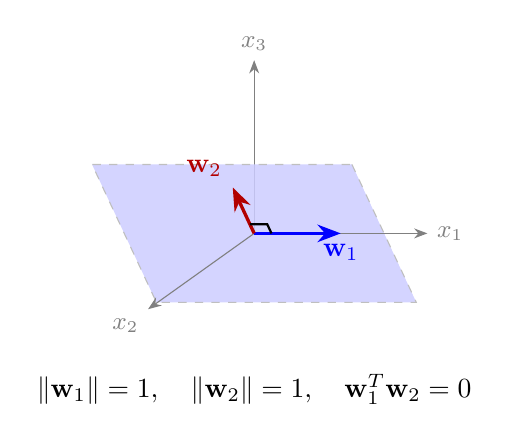
\begin{tikzpicture}[scale=1.1, >=Stealth,
  x={(1cm,0cm)}, y={(-0.35cm,-0.25cm)}, z={(0cm,1cm)}]
% 3D projection: x₁→right, x₂→lower-left (into page), x₃→up
% w1 = (1, 0, 0),  w2 = (0, 0.707, 0.707)
% Parallelogram vertices at ±1.5·w1 ± 1.5·w2, centered at origin
\coordinate (A) at ( 1.5,  1.061,  1.061);  %  1.5w1 + 1.5w2
\coordinate (B) at ( 1.5, -1.061, -1.061);  %  1.5w1 - 1.5w2
\coordinate (C) at (-1.5, -1.061, -1.061);  % -1.5w1 - 1.5w2
\coordinate (D) at (-1.5,  1.061,  1.061);  % -1.5w1 + 1.5w2
% --- Layer 1: x₃ axis BEHIND the plane (will be partially occluded)
\draw[gray, thin, ->] (0,0,0) -- (0,0,2) node[above] {\small $x_3$};
% --- Layer 2: the plane (occludes x₃ where they overlap)
\fill[blue!20, opacity=0.85] (A) -- (B) -- (C) -- (D) -- cycle;
\draw[gray!50, dashed] (A) -- (B) -- (C) -- (D) -- cycle;
% --- Layer 3: x₁, x₂ axes IN FRONT of the plane
\draw[gray, thin, ->] (0,0,0) -- (2,0,0) node[right] {\small $x_1$};
\draw[gray, thin, ->] (0,0,0) -- (0,3.5,0) node[below left] {\small $x_2$};
% --- Layer 4: vectors and markers (topmost)
\draw[->, very thick, blue] (0,0,0) -- (1,0,0)
  node[below] {$\mathbf{w}_1$};
\draw[->, very thick, red!70!black] (0,0,0) -- (0,0.707,0.707)
  node[above left] {$\mathbf{w}_2$};
\draw[thick] (0.2,0,0) -- (0.2,0.141,0.141) -- (0,0.141,0.141);
% label
\node at (0, 0, -1.8) {$\|\mathbf{w}_1\| = 1, \quad \|\mathbf{w}_2\| = 1, \quad \mathbf{w}_1^T\mathbf{w}_2 = 0$};
\end{tikzpicture}
\end{center}

\vspace{0.3em}

Perpendicular. Unit length. \quad \x{Is there a name for this?}

\end{frame}

% ─── INTERLUDE: ORTHOGONALITY CRASH COURSE ───
%
% ADR: The audience has SEEN two vectors that are perpendicular and unit
% length. They intuit the pattern. NOW we give them the vocabulary to
% name what they see. Discovery-first: see → intuit → name → formalize.
% The interlude is 3 slides: inner product, orthogonal, orthonormal.

% ADR: Recall the inner product. Needed to formalize "perpendicular"
% (dot product = 0) and "unit length" (dot product with self = 1).
% AUDIENCE EMOTION: "ok, I remember — dot product measures angle"
% AUDIENCE ATTENTION: moderate — review, but anchored by what they just saw.
\begin{frame}{Recall: The Inner Product}

The \x{inner product} (dot product) of two vectors $\mathbf{u}, \mathbf{v} \in \mathbb{R}^n$:

$$\mathbf{u}^T \mathbf{v} = u_1 v_1 + u_2 v_2 + \cdots + u_n v_n$$

\vspace{0.3em}

\x{Two key uses}:

\vspace{0.3em}

\begin{itemize}
\item \x{Length}: $\|\mathbf{u}\| = \sqrt{\mathbf{u}^T \mathbf{u}}$

\vspace{0.3em}

\item \x{Angle}: $\mathbf{u}^T \mathbf{v} = \|\mathbf{u}\| \, \|\mathbf{v}\| \cos\theta$

\vspace{0.3em}

In particular: $\mathbf{u}^T \mathbf{v} = 0 \iff \theta = 90°$ \quad (perpendicular!)
\end{itemize}

\end{frame}

% ADR: Define orthogonal. One-line definition + TikZ diagram echoing
% the 3D picture they saw. Now they have the NAME for what they intuited.
% AUDIENCE EMOTION: "orthogonal = perpendicular — that's what w₁, w₂ were"
\begin{frame}{Orthogonal Vectors}

\begin{defi}[Orthogonal]
Two vectors $\mathbf{u}$ and $\mathbf{v}$ are \x{orthogonal} if $\mathbf{u}^T \mathbf{v} = 0$.
\end{defi}

\vspace{0.3em}

\begin{center}
\begin{tikzpicture}[scale=1.2, >=Stealth]
\draw[->, thick, blue] (0,0) -- (2.5,0) node[right] {$\mathbf{u}$};
\draw[->, thick, red!70!black] (0,0) -- (0,2) node[above] {$\mathbf{v}$};
\draw[thick] (0.3,0) -- (0.3,0.3) -- (0,0.3);
\node at (1.2, -0.6) {$\mathbf{u}^T \mathbf{v} = 0$};
\end{tikzpicture}
\end{center}

\vspace{0.3em}

Orthogonal $=$ perpendicular $=$ ``no overlap in direction.''

\end{frame}

% ADR: Define orthonormal. Two conditions: orthogonal + unit length.
% The δᵢⱼ notation is compact and used in the theorem later.
% AUDIENCE EMOTION: "orthonormal = perpendicular + unit. Now I have the word"
% AUDIENCE ATTENTION: checklist format primes them for verification.
\begin{frame}{Orthonormal Vectors}

\begin{defi}[Orthonormal Set]
Vectors $\mathbf{w}_1, \ldots, \mathbf{w}_r$ are \x{orthonormal} if:
\begin{enumerate}
\item \x{Orthogonal}: $\mathbf{w}_i^T \mathbf{w}_j = 0$ for all $i \neq j$ \quad (perpendicular pairs)
\item \x{Unit length}: $\|\mathbf{w}_i\| = 1$ for all $i$
\end{enumerate}
\end{defi}

\vspace{0.3em}

Compact notation: $\mathbf{w}_i^T \mathbf{w}_j = \delta_{ij} = \begin{cases} 1 & i = j \\ 0 & i \neq j \end{cases}$

\vspace{0.5em}

An \x{orthonormal basis} of a subspace $S$: an orthonormal set that also \x{spans} $S$.

\end{frame}

% ─── RETURN TO CROSS-FILLING ───
%
% ADR: Come back to the example. Restate vectors (audience has no memory!)
% and CHECK the orthonormality conditions one by one. Add the third check:
% "span Col(P)?" — because orthonormal BASIS requires spanning.
% AUDIENCE EMOTION: "our vectors ARE orthonormal! cross-filling did this!"
% AUDIENCE ATTENTION: satisfying closure — three checks, three checkmarks.
% WHY RESTATE: 3 definition slides have passed. Vectors are gone from
% working memory. Restate P = w₁w₁^T + w₂w₂^T and the vectors themselves.
\begin{frame}{Back to Our Vectors --- They Are Orthonormal!}

Recall: diagonal cross-filling gave us $P = \mathbf{w}_1\mathbf{w}_1^T + \mathbf{w}_2\mathbf{w}_2^T$ with

$$\mathbf{w}_1 = \begin{pmatrix} 1 \\ 0 \\ 0 \end{pmatrix}, \qquad \mathbf{w}_2 = \begin{pmatrix} 0 \\ \frac{1}{\sqrt{2}} \\ \frac{1}{\sqrt{2}} \end{pmatrix}$$

\vspace{0.3em}

\x{Unit length?} \quad $\|\mathbf{w}_1\|^2 = 1 \;\checkmark$ \qquad $\|\mathbf{w}_2\|^2 = \tfrac{1}{2} + \tfrac{1}{2} = 1 \;\checkmark$

\vspace{0.3em}

\x{Orthogonal?} \quad $\mathbf{w}_1^T \mathbf{w}_2 = 1 \cdot 0 + 0 \cdot \tfrac{1}{\sqrt{2}} + 0 \cdot \tfrac{1}{\sqrt{2}} = 0 \;\checkmark$

\vspace{0.3em}

\x{Span $\operatorname{Col}(P)$?} \quad $P = \mathbf{w}_1\mathbf{w}_1^T + \mathbf{w}_2\mathbf{w}_2^T$ \;\checkmark \quad (every $P\mathbf{x}$ is a combination of $\mathbf{w}_1, \mathbf{w}_2$)

\vspace{0.5em}

$\mathbf{w}_1, \mathbf{w}_2$ is an \x{orthonormal basis} of $\operatorname{Col}(P)$ --- \x{for free}!

\end{frame}

% ADR: NOW state the theorem. The audience has SEEN the result in a concrete
% example: symmetric pieces, orthonormal vectors, decomposition. The theorem
% formalizes what they already believe. This mirrors §1→§2: discover, THEN
% state. The "Why orthonormal?" explanation corrects the naive intuition
% "V = U^T" — the actual relationship involves pivot scaling, but the
% conclusion (orthonormality) follows from VU = I combined with symmetry.
% AUDIENCE EMOTION: "the theorem matches exactly what I just saw"
% AUDIENCE ATTENTION: the formal statement is anchored by the concrete memory.
% ADR: State the theorem cleanly on its own slide. The "why" comes after.
% AUDIENCE EMOTION: "the theorem matches what I just saw"
% AUDIENCE ATTENTION: the formal statement is anchored by the concrete memory.
\begin{frame}{The Theorem}

\begin{thm}[Diagonal Cross-Filling of Orthogonal Projections]
Let $P$ be an orthogonal projection ($P^2 = P$, $P^T = P$) of rank $r$.

Diagonal cross-filling decomposes $P$ into:
$$P = \mathbf{w}_1\mathbf{w}_1^T + \mathbf{w}_2\mathbf{w}_2^T + \cdots + \mathbf{w}_r\mathbf{w}_r^T$$
where $\mathbf{w}_1, \ldots, \mathbf{w}_r$ is an \x{orthonormal basis} of $\operatorname{Col}(P)$.
\end{thm}

\vspace{1em}

We verified this for our $3 \times 3$ example. But \x{why} must it always work?

\end{frame}

% ADR: Show P = WW^T concretely. All three matrices written out with
% underbrace labels. Columns of W colored blue/red for piece 1/2,
% rows of W^T colored to match. The audience sees the SYMMETRIC
% factorization — no U, no V, only W and w.
% AUDIENCE EMOTION: "P factors as WW^T — both sides are the same matrix!"
% AUDIENCE ATTENTION: three concrete matrices with color and underbrace.
\begin{frame}{Step 1: Write $P = WW^T$}

Recall: $\mathbf{w}_i = \text{column}_i / \sqrt{\text{pivot}_i}$. \quad Stack them into $W$:

$$\underbrace{\begin{pmatrix}
\bl{1} & \rd{0} \\[2pt]
\bl{0} & \rd{\frac{1}{\sqrt{2}}} \\[2pt]
\bl{0} & \rd{\frac{1}{\sqrt{2}}}
\end{pmatrix}}_{W\;=\;(\,\bl{\mathbf{w}_1}\;\;\rd{\mathbf{w}_2}\,)}
\underbrace{\begin{pmatrix}
\bl{1} & \bl{0} & \bl{0} \\[2pt]
\rd{0} & \rd{\frac{1}{\sqrt{2}}} & \rd{\frac{1}{\sqrt{2}}}
\end{pmatrix}}_{W^T\;=\;\left(\begin{smallmatrix} \bl{\mathbf{w}_1^T} \\ \rd{\mathbf{w}_2^T} \end{smallmatrix}\right)}
=
\underbrace{\begin{pmatrix}
1 & 0 & 0 \\[2pt]
0 & \frac{1}{2} & \frac{1}{2} \\[2pt]
0 & \frac{1}{2} & \frac{1}{2}
\end{pmatrix}}_{P}$$

\vspace{0.5em}

$P = \bl{\mathbf{w}_1}\bl{\mathbf{w}_1^T} + \rd{\mathbf{w}_2}\rd{\mathbf{w}_2^T}$ \quad --- same $W$ on \x{both} sides.

\end{frame}

% ADR: Compute W^TW concretely with colored matrices and underbrace.
% The audience SEES the identity matrix appear. Then explain WHY:
% P² = P forces W^TW = I. No U, no V — only W.
% AUDIENCE EMOTION: "W^TW = I — the columns of W are orthonormal!"
% AUDIENCE ATTENTION: colored matrix product → clean I₂.
\begin{frame}{Step 2: $W^TW = I$}

$$\underbrace{\begin{pmatrix}
\bl{1} & \bl{0} & \bl{0} \\[2pt]
\rd{0} & \rd{\frac{1}{\sqrt{2}}} & \rd{\frac{1}{\sqrt{2}}}
\end{pmatrix}}_{W^T}
\underbrace{\begin{pmatrix}
\bl{1} & \rd{0} \\[2pt]
\bl{0} & \rd{\frac{1}{\sqrt{2}}} \\[2pt]
\bl{0} & \rd{\frac{1}{\sqrt{2}}}
\end{pmatrix}}_{W}
=
\underbrace{\begin{pmatrix}
\bl{1} & 0 \\[2pt]
0 & \rd{1}
\end{pmatrix}}_{I_2} \quad\checkmark$$

\vspace{0.5em}

\x{Why must this hold?} \quad $P^2 = P$:
$$WW^T \!\cdot\! WW^T = WW^T \;\Longrightarrow\; W\bigl({\color{red}\boldsymbol{W^TW}}\bigr)W^T = W\bigl({\color{red}\boldsymbol{I}}\bigr)W^T$$

Cancel $W$ and $W^T$ from both sides: $\;{\color{red}\boldsymbol{W^TW = I}}$.

\end{frame}

% ADR: QED slide. Expand W^TW = I into concrete colored matrix product,
% just like §2 did for VU = I. Show w_1, w_2 as columns/rows with color,
% compute each entry, arrive at I_2. The audience sees every dot product.
% AUDIENCE EMOTION: "I can see every inner product — they really are orthonormal!"
\begin{frame}{$W^TW = I$ --- Spelled Out}

$$\underbrace{\begin{pmatrix}
\bl{\mathbf{w}_1^T} \\[2pt] \rd{\mathbf{w}_2^T}
\end{pmatrix}}_{W^T}
\underbrace{\begin{pmatrix}
\bl{\mathbf{w}_1} & \rd{\mathbf{w}_2}
\end{pmatrix}}_{W}
=
\begin{pmatrix}
\bl{\mathbf{w}_1^T}\bl{\mathbf{w}_1} & \bl{\mathbf{w}_1^T}\rd{\mathbf{w}_2} \\[4pt]
\rd{\mathbf{w}_2^T}\bl{\mathbf{w}_1} & \rd{\mathbf{w}_2^T}\rd{\mathbf{w}_2}
\end{pmatrix}
=
\underbrace{\begin{pmatrix}
\bl{1} & 0 \\[2pt]
0 & \rd{1}
\end{pmatrix}}_{I_2}$$

\vspace{0.3em}

\x{Diagonal}: $\bl{\mathbf{w}_1^T}\bl{\mathbf{w}_1} = \bl{1}\!\cdot\!\bl{1} + \bl{0}\!\cdot\!\bl{0} + \bl{0}\!\cdot\!\bl{0} = \bl{1}$ \;\checkmark \quad
$\rd{\mathbf{w}_2^T}\rd{\mathbf{w}_2} = \rd{\frac{1}{\sqrt{2}}}\!\cdot\!\rd{\frac{1}{\sqrt{2}}} + \rd{\frac{1}{\sqrt{2}}}\!\cdot\!\rd{\frac{1}{\sqrt{2}}} = \rd{1}$ \;\checkmark

\vspace{0.3em}

\x{Off-diagonal}: $\bl{\mathbf{w}_1^T}\rd{\mathbf{w}_2} = \bl{1}\!\cdot\!\rd{0} + \bl{0}\!\cdot\!\rd{\frac{1}{\sqrt{2}}} + \bl{0}\!\cdot\!\rd{\frac{1}{\sqrt{2}}} = 0$ \;\checkmark

\vspace{0.5em}

$\mathbf{w}_1, \mathbf{w}_2$ is an \x{orthonormal basis} of $\operatorname{Col}(P)$ --- \x{for free}! \qed

\vspace{0.3em}

\x{Summary}: $P^T\!=\!P \;\Longrightarrow\; P = WW^T$; \quad $P^2\!=\!P \;\Longrightarrow\; W^TW = I$ (orthonormal).

\end{frame}

% ── Example: Orthonormal basis of Null(P) via cross-filling I−P ──

% ADR: Transition from Col(P) to Null(P). The audience just learned to
% find orthonormal bases of Col(P). The natural next question is: what
% about Null(P)? This motivates the trick: Null(P) = Col(I−P).
% AUDIENCE EMOTION: "we can do Col — but how about Null?"
% AUDIENCE ATTENTION: the open question creates curiosity.
\begin{frame}{$\operatorname{Col}(P)$ \checkmark\ --- What About $\operatorname{Null}(P)$?}

We just showed: diagonal cross-fill an orthogonal projection $P$

$$\Longrightarrow \quad \text{orthonormal basis of } \operatorname{Col}(P).$$

\vspace{0.5em}

\x{New question}: Can we find an orthonormal basis of $\operatorname{Null}(P)$?

\end{frame}

% ADR: Give P concretely. The audience needs to see the matrix before any
% trick is revealed. State rank and the task clearly.
% AUDIENCE EMOTION: "ok, here's the problem — how do I start?"
\begin{frame}{Exercise}

$$P = \begin{pmatrix} \frac{1}{4} & \frac{1}{4} & \frac{1}{4} & \frac{1}{4} \\[3pt] \frac{1}{4} & \frac{1}{4} & \frac{1}{4} & \frac{1}{4} \\[3pt] \frac{1}{4} & \frac{1}{4} & \frac{1}{4} & \frac{1}{4} \\[3pt] \frac{1}{4} & \frac{1}{4} & \frac{1}{4} & \frac{1}{4} \end{pmatrix}$$

$P$ is an orthogonal projection ($P^2 = P$, $P^T = P$), $\operatorname{rank}(P) = 1$.

\vspace{0.5em}

\x{Task}: Find an orthonormal basis of $\operatorname{Null}(P)$.

\end{frame}

% ADR: Reveal the trick: Null(P) = Col(I−P), and I−P is also an orthogonal
% projection. So we just cross-fill I−P! Write out Q concretely.
% AUDIENCE EMOTION: "oh! just cross-fill I−P — same method!"
\begin{frame}{The Trick: $\operatorname{Null}(P) = \operatorname{Col}(I - P)$}

$Q = I - P$ is also an orthogonal projection ($Q^2 = Q$, $Q^T = Q$), rank $= 3$.

$$Q = I - P = \begin{pmatrix} \frac{3}{4} & -\frac{1}{4} & -\frac{1}{4} & -\frac{1}{4} \\[3pt] -\frac{1}{4} & \frac{3}{4} & -\frac{1}{4} & -\frac{1}{4} \\[3pt] -\frac{1}{4} & -\frac{1}{4} & \frac{3}{4} & -\frac{1}{4} \\[3pt] -\frac{1}{4} & -\frac{1}{4} & -\frac{1}{4} & \frac{3}{4} \end{pmatrix}$$

\vspace{0.3em}

Cross-fill $Q$ $\;\Longrightarrow\;$ orthonormal basis of $\operatorname{Col}(Q) = \operatorname{Null}(P)$.

\end{frame}

% ADR: Step 1 — cross-fill Q at (1,1). Show the 4×4 matrix with cross
% highlighted. Extract column and pivot, compute w₁ = col/√pivot.
% AUDIENCE EMOTION: "same procedure — I know what to do"
% AUDIENCE ATTENTION: the blue cross in the 4×4 matrix is eye-catching.
\begin{frame}{Cross-Fill $Q$: Step 1}

\x{Pivot} at $(\pvt{1},\pvt{1})$, value $= \pvt{\frac{3}{4}}$:

$$Q = \begin{pmatrix} \pvt{\frac{3}{4}} & \crs{-\frac{1}{4}} & \crs{-\frac{1}{4}} & \crs{-\frac{1}{4}} \\[3pt] \crs{-\frac{1}{4}} & \frac{3}{4} & -\frac{1}{4} & -\frac{1}{4} \\[3pt] \crs{-\frac{1}{4}} & -\frac{1}{4} & \frac{3}{4} & -\frac{1}{4} \\[3pt] \crs{-\frac{1}{4}} & -\frac{1}{4} & -\frac{1}{4} & \frac{3}{4} \end{pmatrix}$$

$\text{col} = \left(\begin{smallmatrix} \crs{3/4} \\ \crs{-1/4} \\ \crs{-1/4} \\ \crs{-1/4} \end{smallmatrix}\right)$, \quad $\text{pivot} = \pvt{\frac{3}{4}}$ \qquad $\Longrightarrow$ \qquad $\bl{\mathbf{w}_1} = \dfrac{\text{col}}{\sqrt{3/4}} = \begin{pmatrix} \bl{\frac{\sqrt{3}}{2}} \\[3pt] \bl{-\frac{\sqrt{3}}{6}} \\[3pt] \bl{-\frac{\sqrt{3}}{6}} \\[3pt] \bl{-\frac{\sqrt{3}}{6}} \end{pmatrix}$

\end{frame}

% ADR: Step 2 — cross-fill the remainder at (2,2). Ghost the (1,1)-cross.
% Show remainder with cross highlighted, extract w₂.
% AUDIENCE EMOTION: "same pattern again"
\begin{frame}{Cross-Fill $Q$: Step 2}

\x{Pivot} at $(\pvt{2},\pvt{2})$ in the remainder, value $= \pvt{\frac{2}{3}}$:

$$Q - R_1 = \begin{pmatrix} \ghost{0} & \ghost{0} & \ghost{0} & \ghost{0} \\[3pt] \ghost{0} & \pvt{\frac{2}{3}} & \crs{-\frac{1}{3}} & \crs{-\frac{1}{3}} \\[3pt] \ghost{0} & \crs{-\frac{1}{3}} & \frac{2}{3} & -\frac{1}{3} \\[3pt] \ghost{0} & \crs{-\frac{1}{3}} & -\frac{1}{3} & \frac{2}{3} \end{pmatrix}$$

$\text{col} = \left(\begin{smallmatrix} \crs{0} \\ \crs{2/3} \\ \crs{-1/3} \\ \crs{-1/3} \end{smallmatrix}\right)$, \quad $\text{pivot} = \pvt{\frac{2}{3}}$ \qquad $\Longrightarrow$ \qquad $\rd{\mathbf{w}_2} = \dfrac{\text{col}}{\sqrt{2/3}} = \begin{pmatrix} \rd{0} \\[3pt] \rd{\frac{\sqrt{6}}{3}} \\[3pt] \rd{-\frac{\sqrt{6}}{6}} \\[3pt] \rd{-\frac{\sqrt{6}}{6}} \end{pmatrix}$

\end{frame}

% ADR: Step 3 — cross-fill the remainder at (3,3). Ghost rows 1-2.
% Extract w₃. Last step — remainder becomes zero.
% AUDIENCE EMOTION: "one more — and we're done"
\begin{frame}{Cross-Fill $Q$: Step 3}

\x{Pivot} at $(\pvt{3},\pvt{3})$ in the remainder, value $= \pvt{\frac{1}{2}}$:

$$Q - R_1 - R_2 = \begin{pmatrix} \ghost{0} & \ghost{0} & \ghost{0} & \ghost{0} \\[3pt] \ghost{0} & \ghost{0} & \ghost{0} & \ghost{0} \\[3pt] \ghost{0} & \ghost{0} & \pvt{\frac{1}{2}} & \crs{-\frac{1}{2}} \\[3pt] \ghost{0} & \ghost{0} & \crs{-\frac{1}{2}} & \frac{1}{2} \end{pmatrix}$$

$\text{col} = \left(\begin{smallmatrix} \crs{0} \\ \crs{0} \\ \crs{1/2} \\ \crs{-1/2} \end{smallmatrix}\right)$, \quad $\text{pivot} = \pvt{\frac{1}{2}}$ \qquad $\Longrightarrow$ \qquad $\tl{\mathbf{w}_3} = \dfrac{\text{col}}{\sqrt{1/2}} = \begin{pmatrix} \tl{0} \\[3pt] \tl{0} \\[3pt] \tl{\frac{1}{\sqrt{2}}} \\[3pt] \tl{-\frac{1}{\sqrt{2}}} \end{pmatrix}$

\end{frame}

% ADR: Result slide. Show W^TW = I₃ with colored symbolic matrices and
% underbrace, then concrete verification of a diagonal and off-diagonal
% entry. Conclude: orthonormal basis of Null(P).
% AUDIENCE EMOTION: "it works — three orthonormal vectors, for free!"
\begin{frame}{$W^TW = I$ --- Orthonormal Basis of $\operatorname{Null}(P)$}

$$\underbrace{\begin{pmatrix} \bl{\mathbf{w}_1^T} \\[2pt] \rd{\mathbf{w}_2^T} \\[2pt] \tl{\mathbf{w}_3^T} \end{pmatrix}}_{W^T}
\underbrace{\begin{pmatrix} \bl{\mathbf{w}_1} & \rd{\mathbf{w}_2} & \tl{\mathbf{w}_3} \end{pmatrix}}_{W}
=
\underbrace{\begin{pmatrix} \bl{1} & 0 & 0 \\[2pt] 0 & \rd{1} & 0 \\[2pt] 0 & 0 & \tl{1} \end{pmatrix}}_{I_3} \quad\checkmark$$

\vspace{0.3em}

\x{Verify}: $\|\bl{\mathbf{w}_1}\|^2 = \frac{3}{4} + \frac{1}{12} + \frac{1}{12} + \frac{1}{12} = 1$ \;\checkmark \qquad $\bl{\mathbf{w}_1^T}\rd{\mathbf{w}_2} = 0 - \frac{\sqrt{18}}{18} + \frac{\sqrt{18}}{36} + \frac{\sqrt{18}}{36} = 0$ \;\checkmark

\vspace{0.5em}

$\bl{\mathbf{w}_1}, \rd{\mathbf{w}_2}, \tl{\mathbf{w}_3}$ is an \x{orthonormal basis} of $\operatorname{Null}(P)$ --- \x{for free}!

\end{frame}

% ═══════════════════════════════════════
% §5 WHAT IF UV = I?
% ═══════════════════════════════════════
% ADR: §2 showed P=UV, P²=P → VU=I (projection → identity). The natural
% reverse question: UV=I → VU=? Answer: VU is a projection. Then rank=trace
% pins down rank(VU)=n, giving three cases by shape: thin×fat impossible,
% square×square → VU=I, fat×thin → genuine projection.
% This section bridges projection theory to general linear algebra.
\section{What If $UV = I$?}

% ADR: Motivation — the "reverse question." §2 went projection → identity.
% Now reverse: identity → what? The symmetry makes the audience curious.
% AUDIENCE EMOTION: "we went one way — what happens going back?"
% AUDIENCE ATTENTION: the question format is engaging.
\begin{frame}{The Reverse Question}

In \S2 we discovered:

$$P = UV, \quad P^2 = P \quad\Longrightarrow\quad VU = I_r$$

Projection $\longrightarrow$ identity.

\vspace{0.5em}

\x{Reverse}: Suppose we \x{start} with $UV = I_n$.

\vspace{0.3em}

What is $VU$?

\end{frame}

% ADR: The punchline — VU is always a projection. One-line proof.
% The circle closes: projection → identity → projection.
% AUDIENCE EMOTION: "it comes back to projections — beautiful!"
\begin{frame}{$VU$ Is Always a Projection}

\begin{thm}
If $UV = I_n$ ($U$ is $n \times r$, $V$ is $r \times n$), then $(VU)^2 = VU$.
\end{thm}

\vspace{0.3em}

\textbf{Proof}:
$$(VU)(VU) = V\underbrace{(UV)}_{=\, I_n}U = VU \qquad\qed$$

\vspace{0.5em}

The circle closes:

$$\text{Projection} \;\xrightarrow{\;\text{\S2}\;}\; \text{Identity} \;\xrightarrow{\;\text{reverse}\;}\; \text{Projection}$$

\end{frame}

% ADR: Use rank = trace (§3) to pin down rank(VU) = n. The cyclic property
% of trace is the key. The audience sees §3's result strike in a new context.
% AUDIENCE EMOTION: "rank = trace strikes again!"
\begin{frame}{The Rank Is Determined}

$VU$ is an $r \times r$ projection. By rank $=$ trace (\S3):

$$\operatorname{rank}(VU) = \operatorname{trace}(VU) = \operatorname{trace}(UV) = \operatorname{trace}(I_n) = \x{n}$$

\vspace{0.5em}

So $VU$ is an $r \times r$ projection of rank $n$.

\vspace{0.3em}

Since rank $\leq$ size: \quad $n \leq r$.

\end{frame}

% ADR: Three cases by comparing r and n. TikZ shows matrix shapes for each
% case in a horizontal triptych. U is always blue!15, V is always red!15
% (matching the UV product convention). The impossible cases (r<n and
% r>n in the ⇒ proof later) get red diagonal X-crosses. The r=n case
% shows two equal squares side by side — visually "they fit."
% The r>n case shows fat U and thin V separated (not overlapping!) so
% the audience sees distinct shapes. Below each diagram: one-line verdict.
% AUDIENCE EMOTION: "three clean cases — the shapes tell the story"
% AUDIENCE ATTENTION: the visual rectangles make the dimension argument visceral.
\begin{frame}{Three Cases by Shape}

$U$ is $n \times r$, \; $V$ is $r \times n$, \; $UV = I_n$, \; and $n \leq r$.

\vspace{0.3em}

\begin{center}
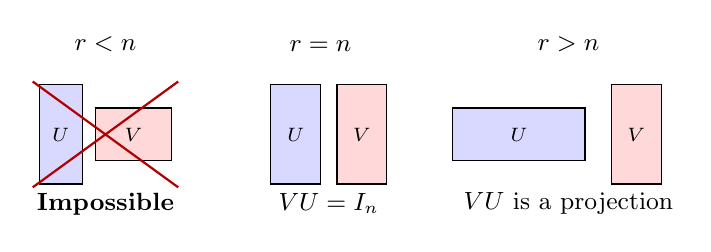
\begin{tikzpicture}[scale=0.42, >=Stealth]
% Case 1: r < n — impossible
\node[above] at (2.5,3.7) {\small $r < n$};
\draw[fill=blue!15] (0.5,0) rectangle (1.8,3);
\node at (1.15,1.5) {\scriptsize $U$};
\draw[fill=red!15] (2.2,0.7) rectangle (4.5,2.3);
\node at (3.35,1.5) {\scriptsize $V$};
\node at (2.5,-0.6) {\small\x{Impossible}};
\draw[thick, red!70!black] (0.3,-0.1) -- (4.7,3.1);
\draw[thick, red!70!black] (0.3,3.1) -- (4.7,-0.1);

% Case 2: r = n — square
\node[above] at (9,3.7) {\small $r = n$};
\draw[fill=blue!15] (7.5,0) rectangle (9,3);
\node at (8.25,1.5) {\scriptsize $U$};
\draw[fill=red!15] (9.5,0) rectangle (11,3);
\node at (10.25,1.5) {\scriptsize $V$};
\node at (9.25,-0.6) {\small $VU = I_n$};

% Case 3: r > n — fat × thin (separated)
\node[above] at (16.5,3.7) {\small $r > n$};
\draw[fill=blue!15] (13,0.7) rectangle (17,2.3);
\node at (15,1.5) {\scriptsize $U$};
\draw[fill=red!15] (17.8,0) rectangle (19.3,3);
\node at (18.55,1.5) {\scriptsize $V$};
\node at (16.5,-0.6) {\small $VU$ is a projection};
\end{tikzpicture}
\end{center}

\vspace{0.2em}

\begin{itemize}
\item $r < n$ (thin $\times$ fat): rank$(VU) \leq r < n$ --- contradicts rank $= n$. \;\x{Impossible.}
\item $r = n$ (square $\times$ square): rank-$n$ projection on $\mathbb{R}^n$ $\;\Longrightarrow\;$ $VU = I_n$.
\item $r > n$ (fat $\times$ thin): $VU$ is a \x{genuine} rank-$n$ projection on $\mathbb{R}^r$.
\end{itemize}

\end{frame}

% ADR: The square case gives one-sided ⇒ two-sided. This resolves the
% Lecture 1 promise: we defined invertible with BOTH AB=I and BA=I, and
% now show one suffices. The proof is a one-liner from the three-case analysis.
% AUDIENCE EMOTION: "finally — the Lecture 1 promise is fulfilled"
% AUDIENCE ATTENTION: the Lecture 1 callback triggers memory and closure.
\begin{frame}{The Square Case: One-Sided $\Rightarrow$ Two-Sided}

\begin{cor}
If $U, V$ are both $n \times n$ and $UV = I_n$, then $VU = I_n$.
\end{cor}

\textbf{Proof}: $VU$ is an $n \times n$ projection of rank $n$ (the square case).

A full-rank projection must be $I$ (proved in Lecture 7; quick reminder if needed):

$I_n - VU$ is also a projection, and
$$\operatorname{rank}(I_n - VU) = \operatorname{trace}(I_n - VU) = n - n = 0 \;\;\Longrightarrow\;\; VU = I_n. \qquad\qed$$

\vspace{0.3em}

\x{Recall Lecture 1}: We defined ``invertible'' by requiring \x{both} $AB = I$ and $BA = I$.

Now we know: for square matrices, \x{one equation suffices}!

$$UV = I_n \quad\Longrightarrow\quad VU = I_n$$

\end{frame}

% ═══════════════════════════════════════
% §6 FULL RANK ⟺ INVERTIBLE
% ═══════════════════════════════════════
% ADR: The capstone theorem — full rank ↔ invertible. Uses the square case
% from §5 plus the augmented/stacked matrix trick. This is the major
% application of everything built in §1-§5.
\section{Full Rank $\iff$ Invertible}

% ADR: Motivation — §5 gave us the one-sided ⇒ two-sided tool. The natural
% next question: when IS a matrix invertible? This frames the capstone theorem.
% AUDIENCE EMOTION: "§5 gave a tool — now what can we DO with it?"
% AUDIENCE ATTENTION: the question primes for the big theorem.
\begin{frame}{When Is a Matrix Invertible?}

\S5 gave us a powerful tool:

$$UV = I_n \;\text{(square)} \quad\Longrightarrow\quad VU = I_n$$

One-sided inverse $\Rightarrow$ two-sided. \quad But \x{when} does a matrix have an inverse?

\vspace{0.5em}

\x{Answer}: Exactly when it has \x{full rank}.

\end{frame}

% ADR: Theorem statement — standalone, clean. Let the audience absorb it.
% AUDIENCE EMOTION: "this is a big theorem"
% AUDIENCE ATTENTION: high — fundamental result, short and clear.
\begin{frame}{Full Rank $\iff$ Invertible}

\begin{thm}[Full Rank $\iff$ Invertible]
An $n \times n$ matrix $X$ is invertible if and only if $\operatorname{rank}(X) = n$.
\end{thm}

\end{frame}

% ADR: ⇒ direction proof with matrix shape diagrams. Reuse the SAME
% TikZ triptych style from §5's "Three Cases" slide: blue!15 for the
% left factor, red!15 for the right factor, red diagonal X-crosses on
% the impossible cases. This visual callback reinforces the §5 framework.
% The audience recognizes the format: "same three cases, now applied."
% k < n is ruled out by §5 (rank argument), k > n by rank(X) ≤ n.
% Only k = n survives.
% AUDIENCE EMOTION: "the three cases from §5 do the work!"
% AUDIENCE ATTENTION: TikZ shapes make the dimension argument visceral.
\begin{frame}{Invertible $\Rightarrow$ Full Rank}

Suppose $XY = I_n$. Cross-fill $X = UV$ with $\operatorname{rank}(X) = k$.

Then $\underbrace{U}_{n \times k}\underbrace{(VY)}_{k \times n} = I_n$. \quad Recall \S5's three cases:

\vspace{0.2em}

\begin{center}
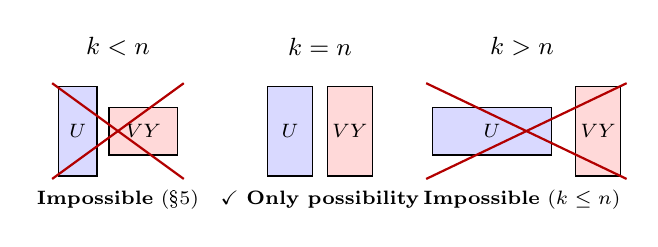
\begin{tikzpicture}[scale=0.38, >=Stealth]
% Case 1: k < n — thin × fat
\node[above] at (2.5,3.7) {\small $k < n$};
\draw[fill=blue!15] (0.5,0) rectangle (1.8,3);
\node at (1.15,1.5) {\scriptsize $U$};
\draw[fill=red!15] (2.2,0.7) rectangle (4.5,2.3);
\node at (3.35,1.5) {\scriptsize $VY$};
\draw[thick, red!70!black] (0.3,-0.1) -- (4.7,3.1);
\draw[thick, red!70!black] (0.3,3.1) -- (4.7,-0.1);
\node at (2.5,-0.8) {\scriptsize\x{Impossible} (\S5)};

% Case 2: k = n — square
\node[above] at (9.25,3.7) {\small $k = n$};
\draw[fill=blue!15] (7.5,0) rectangle (9,3);
\node at (8.25,1.5) {\scriptsize $U$};
\draw[fill=red!15] (9.5,0) rectangle (11,3);
\node at (10.25,1.5) {\scriptsize $VY$};
\node at (9.25,-0.8) {\scriptsize $\checkmark$ \x{Only possibility}};

% Case 3: k > n — fat × thin
\node[above] at (16,3.7) {\small $k > n$};
\draw[fill=blue!15] (13,0.7) rectangle (17,2.3);
\node at (15,1.5) {\scriptsize $U$};
\draw[fill=red!15] (17.8,0) rectangle (19.3,3);
\node at (18.55,1.5) {\scriptsize $VY$};
\draw[thick, red!70!black] (12.8,-0.1) -- (19.5,3.1);
\draw[thick, red!70!black] (12.8,3.1) -- (19.5,-0.1);
\node at (16,-0.8) {\scriptsize\x{Impossible} ($k \leq n$)};
\end{tikzpicture}
\end{center}

\vspace{0.2em}

\begin{itemize}
\item $k < n$: \S5 says this \x{cannot} produce $I_n$ --- ruled out.
\item $k > n$: But $k = \operatorname{rank}(X) \leq n$ for an $n \times n$ matrix --- ruled out.
\item $k = n$: The \x{only} surviving case. $\quad\Longrightarrow\quad \operatorname{rank}(X) = n$. $\checkmark$
\end{itemize}

\end{frame}

% ADR: The clever trick — cross-fill (X | Iₙ) with the SAME pivots as X.
% This produces UW = Iₙ, which by the one-sided inverse proposition gives
% WU = Iₙ, proving U is invertible. Split into two slides (U invertible,
% then V invertible) because doing both on one slide is too dense.
% AUDIENCE EMOTION: "that's a clever move — augmenting to get the inverse"
% AUDIENCE ATTENTION: the boldface step labels keep the argument navigable.
\begin{frame}{Full Rank $\Rightarrow$ Invertible (Part 1: $U$ is invertible)}

\x{($\Leftarrow$) Full rank $\Rightarrow$ invertible}:

Suppose $\operatorname{rank}(X) = n$. Cross-fill $X = UV$ (both $n \times n$).

\vspace{0.5em}

\x{Step 1}: Cross-fill the augmented matrix $(X \mid I_n)$ with the \x{same pivots}:

$$(X \mid I_n) = U(V \mid W)$$

Comparing: $X = UV$ and $I_n = UW$.

\vspace{0.5em}

\x{Step 2}: $UW = I_n$ (both $n \times n$), so by \S5 Corollary: $WU = I_n$.

Therefore $U$ is invertible with $U^{-1} = W$.

\end{frame}

% ADR: Mirror of Part 1 — stack (X; Iₙ) vertically instead of augmenting
% horizontally. Same logic: ZV = Iₙ ⇒ VZ = Iₙ. Then X = UV with both
% invertible gives X⁻¹ = V⁻¹U⁻¹. The QED closes the capstone theorem.
% AUDIENCE EMOTION: "symmetric argument — makes sense"
% AUDIENCE ATTENTION: the parallel structure (Part 1 ↔ Part 2) is reassuring.
\begin{frame}{Full Rank $\Rightarrow$ Invertible (Part 2: $V$ is invertible)}

\x{Step 3}: Cross-fill the stacked matrix with the same pivots:

$$\begin{pmatrix} X \\ I_n \end{pmatrix} = \begin{pmatrix} U \\ Z \end{pmatrix} V$$

Comparing: $X = UV$ and $I_n = ZV$.

\vspace{0.5em}

$ZV = I_n$ (both $n \times n$), so by \S5 Corollary: $VZ = I_n$.

Therefore $V$ is invertible with $V^{-1} = Z$.

\vspace{0.5em}

\x{Step 4}: $X = UV$ with both invertible, so $X^{-1} = V^{-1}U^{-1}$. \qed

\end{frame}

% ═══════════════════════════════════════
% §7 SUMMARY
% ═══════════════════════════════════════
%
% ADR: Summary serves as the "photograph slide" — the one slide the audience
% screenshots for revision. Six numbered items map to §1-§6, giving a
% mental checklist. Each item is one sentence with the section reference
% in parentheses so the audience can locate details. The ordering follows
% the lecture's narrative arc: discover (§1-§2) → harvest (§3-§4) →
% reverse and generalize (§5-§6).
\section{Summary}

% ADR: Summary lists all results in logical order. Numbered to give the
% audience a mental checklist of what they should take away. This is the
% slide they will photograph or screenshot for revision.
% AUDIENCE EMOTION: "ok, I can see the whole picture now"
% AUDIENCE ATTENTION: scanning mode — they skim for anything they missed.
\begin{frame}{What We Proved Today}

\x{1.\ Cross-filling projections} (\S1--\S2): Each rank-1 piece is a projection; $P = UV$ with $P^2 = P$ forces $VU = I$.

\vspace{0.2em}

\x{2.\ Rank $=$ Trace} (\S3): For any projection: $\operatorname{rank}(P) = \operatorname{trace}(P)$.

\vspace{0.2em}

\x{3.\ Orthogonal projections} (\S4): Diagonal cross-filling produces orthonormal bases of $\operatorname{Col}(P)$ and $\operatorname{Null}(P)$.

\vspace{0.2em}

\x{4.\ $UV = I \;\Rightarrow\; VU$ is a projection} (\S5): Three cases by shape --- impossible ($r < n$), identity ($r = n$), genuine projection ($r > n$).

\vspace{0.2em}

\x{5.\ One-sided $\Rightarrow$ two-sided} (\S5): $UV = I_n$ with square matrices forces $VU = I_n$.

\vspace{0.2em}

\x{6.\ Full Rank $\iff$ Invertible} (\S6): An $n \times n$ matrix is invertible iff rank $= n$.

\end{frame}

% ADR: Preview seeds the next lecture's central question. The audience
% leaves with an open thread: "does decomposition into projections work
% BEYOND cross-filling?" This maintains narrative tension across lectures.
% AUDIENCE EMOTION: curiosity — "I want to know the answer"
% AUDIENCE ATTENTION: the question format is engaging even at end-of-lecture.
\begin{frame}{Preview: Lecture 9}

\x{Lecture 9}: Compatible Projections

\vspace{1em}

Today we proved that \x{cross-filling} a projection produces mutually annihilating rank-1 projections.

\vspace{0.5em}

\x{Does this generalize?}

\vspace{0.5em}

Suppose we write $P = R_1 + \cdots + R_k$ (not necessarily from cross-filling), with $\operatorname{rank}(R_1) + \cdots + \operatorname{rank}(R_k) \leq \operatorname{rank}(P)$.

\vspace{0.5em}

Must each $R_i$ still be a projection? Must $R_i R_j = 0$?

\vspace{1em}

The answer is \x{yes} --- this is the \x{projection decomposition theorem}.

\end{frame}

\end{document}
